\problemname{Mini Minesweeper}
Most people who have sat at a computer without internet access have probably tried playing Minesweeper. Minesweeper is played on a rectangular board with \texttt{RxC} cells whose contents are initially unknown. The player can then click on cells to reveal their contents. Mines have been placed in a number of cells, and if the player clicks on such a cell the game is over. In each cell without a mine there is instead a number indicating how many mines there are in the surrounding cells, i.e. in the cells with which it shares a side or a corner. The idea is that these numbers should be used to figure out where the mines are and thus avoid them.

Rudolf has decided to become a professional Minesweeper player. However, he has not played it before and therefore wants to try an easier version, Mini Minesweeper, which is played on a board of size \texttt{2xN}. He has also downloaded \emph{MinesweeperHaXX3000}, which by exploiting a mysterious bug can reveal the contents of all cells on the lower half of the board. Rudolf still does not feel completely confident, and asks you to write a program that, given the information he obtained, can determine which cells are safe to click.

\section*{Input}
The first and only line contains a string of length $N$ ($1 \leq N \leq 50000$). This describes the lower half of the board, and each character is either an `\texttt{X}', meaning a mine, or an integer $d$, $0 \leq d \leq 5$, describing that there are $d$ mines near the cell.

\section*{Output}
If there is no valid board compatible with the input, the program should output `\texttt{fel}' on a line (note lowercase). Otherwise, output a string of $N$ characters --- `\texttt{S}', `\texttt{O}', or `\texttt{X}' --- describing the cells on the upper half of the board. A cell is described with `\texttt{S}' if the cell cannot contain a mine, `\texttt{X}' if the cell definitely contains a mine, and `\texttt{O}' (a capital `o') if the cell could contain a mine but does not have to. The last alternative means that there is at least one valid board where the cell contains a mine and at least one valid board where it does not, see the figures for further explanation.


\section*{Scoring}
Your solution will be tested on a set of test groups.
To earn points for a group, you must pass all test cases in that group.


\noindent
\begin{tabular}{| l | l | p{12cm} |}
  \hline
  \textbf{Group} & \textbf{Points} & \textbf{Constraints} \\ \hline
  $1$    & $40$       & $1 \leq N \leq 10000$ and \emph{there are no mines in the bottom row}. \\ \hline
  $2$    & $60$       & No additional constraints. \\ \hline
\end{tabular}


\section*{Explanation of Sample 1}

\begin{figure}[h!]
\begin{center}
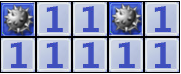
\includegraphics[scale=1]{miniroj1}
\end{center}
\caption{An illustration of one possible solution for the first sample test case.}
\label{fig1}
\end{figure}

\begin{figure}[h!]
\begin{center}
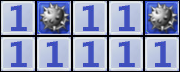
\includegraphics[scale=1]{miniroj2}
\end{center}
\caption{An illustration of the other possible solution for the first sample test case.}
\label{fig1}
\end{figure}
